% PAKETE UND DOKUMENTKONFIGURATION
\documentclass[11pt, a4paper]{scrbook}

% Encoding für Umlaute
\usepackage[utf8]{inputenc}
\usepackage[T1]{fontenc}

% Silbentrennung
\usepackage[ngerman]{babel}

% erweiterte Matheumgebungen und Formelnummer mit Sectionnummer
\usepackage{amsmath}

% zusätzliche mathematische Schriftarten
\usepackage{amsfonts}

% verschiedene mathematische Symbole
\usepackage{amssymb}

% Einheiten setzen z.B. \SI{10}{\kilo\gram\meter\per\second\squared}
% Fehler: \SI{10 +- 0,2e-4}{\metre}
\usepackage{siunitx}
\sisetup{
  output-decimal-marker={,},
  separate-uncertainty
}

% Bilder einfügen
\usepackage{graphicx}

% Textfarbe
\usepackage{color}

% Verweise innerhalb des Dokuments
\usepackage{hyperref}
\hypersetup{
	colorlinks = true,
	allcolors = {black}
}

\newcommand{\vnabla}{\vec{\nabla}}
\newcommand{\ve}{\vec{E}}
\newcommand{\vb}{\vec{B}}
\newcommand{\vh}{\vec{H}}
\newcommand{\vd}{\vec{D}}

\title{Störkörpermessung an Beschleunigungsresonatoren}
\author{Christopher Deutsch}

\begin{document}
	\frontmatter
	\maketitle
	\tableofcontents
	
	\mainmatter
	
	\chapter{Einleitung}
	
	\chapter{Theorie}
	
	\section{Hohlraumresonatoren}
	\begin{figure}[h]
		\centering
		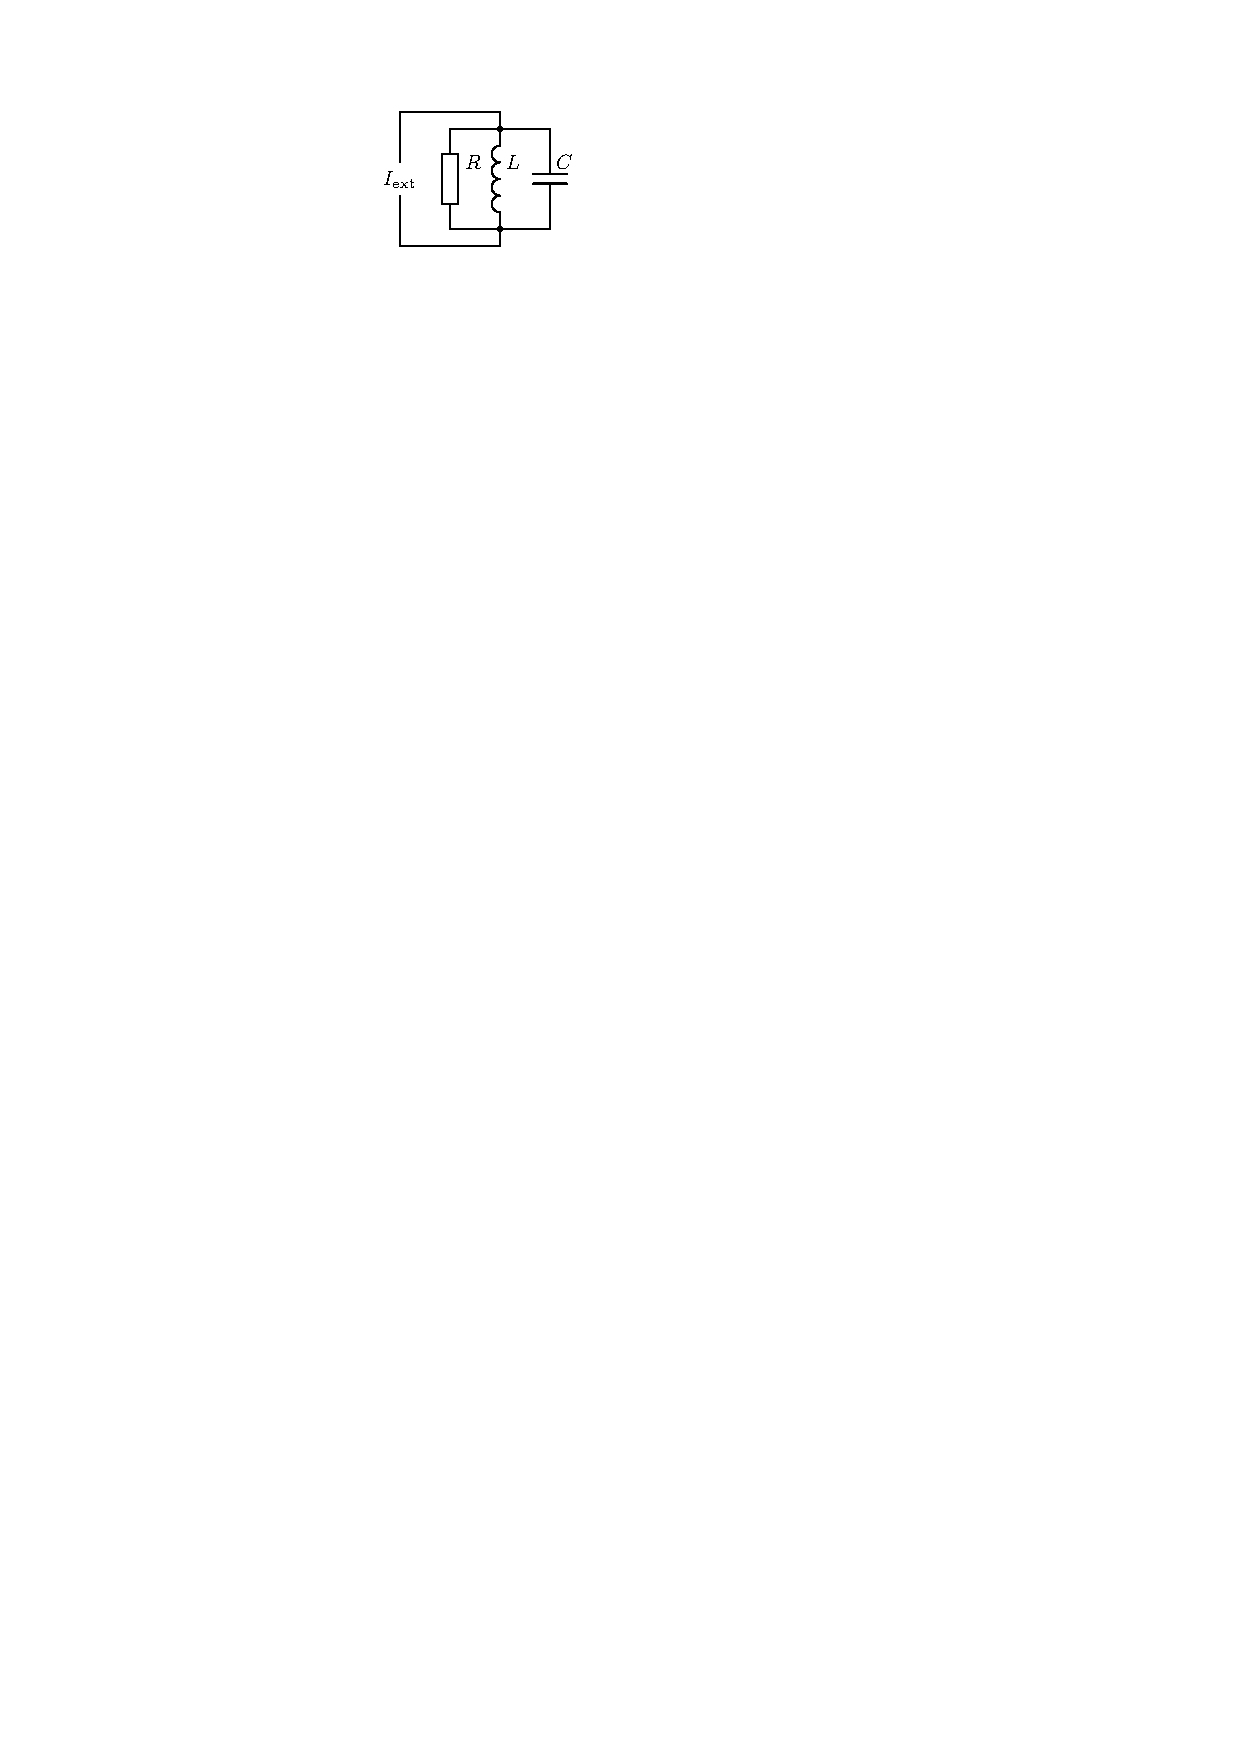
\includegraphics[width=0.35\textwidth]{./figures/RLC_circuit.pdf}
		\caption{RLC Parallelschwingkreis}
		\label{fig:rlc_circuit}
	\end{figure}
	Die elektrischen Eigenschaften von Hohlraumresonatoren in der Nähe einer Resonanz können durch das Modell eines Parallelschwingkreises erklärt werden.
	Die Resonanzfrequenz ist gegeben durch die Thomson'sche Schwingungsgleichung:
	\begin{align}
		\omega_0 = \frac{1}{\sqrt{L C}}
	\end{align}
	(Güte)
	Die Impedanz des Schwingkreises ist gegeben durch:
	\begin{align}
		Z_\mathrm{LCR} = \left( \frac{1}{R} + \frac{1}{i \omega L} + i \omega C \right)
	\end{align}
	Unter der Verwendung der Ausdrücke von Resonanzfrequenz und Güte kann dies geschrieben werden als:
	\begin{align}
		Z_\mathrm{LCR} = \frac{R}{1 + i Q_0 \left( \frac{\omega}{\omega_0}  - \frac{\omega_0}{\omega}\right)}
	\end{align}
	(Maybe Phasensprung, im fall von resonanz reell)
	Durch die magnetische Kopplung wird die Impedanz des Resonators transformiert und wird beschrieben durch:
	\begin{align}
		\kappa = \frac{Z^\prime(\omega_0)}{Z_0}
	\end{align}
	($\kappa < 1$ unterkritisch, $\kappa = 0$ kritisch, $\kappa > 1$ überkritisch)
	wobei $Z^\prime$ die transformierte Impedanz ist und $Z_0$ der Wellenwiderstand des Wellenleiters.
	Ebenfalls wird die zusätzliche Impedanz des Leiters in den Resonator transformiert, was die Güte des Gesamtsystems verändert:
	\begin{align}
		\frac{1}{Q} = \frac{1}{Q_0} + \frac{1}{Q_\mathrm{ext}} \\
		Q_0 = (1 + \kappa) \cdot Q
	\end{align}
	Im folgenden ist der komplexe Reflexionsfaktor $\rho$ von besonderem Interesse:
	\begin{align}
		\rho = \frac{U_{-}}{U_{+}} = \frac{Z^\prime - Z_0}{Z^\prime + Z_0}
	\end{align}
%	($Z^\prime$ transformierte Impedanz, $Z_0$ Wellenwiderstand)
	Es folgt für den Reflexionsfaktor
	\begin{align}
		\rho(\omega) = \frac{(\kappa - 1) + i Q_0 \left( \frac{\omega}{\omega_0}  - \frac{\omega_0}{\omega}\right)}{\left( \kappa + 1 \right) + i Q_0 \left( \frac{\omega}{\omega_0}  - \frac{\omega_0}{\omega}\right)}
	\end{align}
	Mit dem Betrag:
	\begin{align}
		| \rho(\omega) | = \sqrt{\frac{(\kappa - 1)^2 + Q_0^2 \left( \frac{\omega}{\omega_0}  - \frac{\omega_0}{\omega}\right)^2}{(\kappa + 1)^2 + Q_0^2 \left( \frac{\omega}{\omega_0}  - \frac{\omega_0}{\omega}\right)^2}}
	\end{align}
	Damit ist die vom Resonator aufgenommene Leistung:
	\begin{align}
		P_\mathrm{a} = P_0 (1- |\rho|^2)
	\end{align}
	\section{Resonante Störkörpermessung}
	Feld der ungestörten Cavity $\ve_0$ und der gestörten $\ve_1$:
	\begin{subequations}
		\begin{align}
		&\ve_{0,1}(x,y,z,t) = \ve_{0,1}(x,y,z) \, e^{i \omega t} \\
		&\vh_{0,1}(x,y,z,t) = \vh_{0,1}(x,y,z) \, e^{i \omega t}
		\end{align}
	\end{subequations}
	wobei im folgenden mit nur mit den komplexen Amplituden gerechnet wird.
	Mit den Maxwell-Gleichungen:
	\begin{subequations}
		\begin{align}
			&\vnabla \times \ve = - \frac{\partial \vb}{\partial t} \\
			&\vnabla \times \vh = \frac{\partial \vd}{\partial t}
		\end{align}
	\end{subequations}
	folgt nach Elimination der Zeitabhängigkeit:
	\begin{subequations}
		\begin{align}
			&\vnabla \times \ve_{0,1} = - i \omega_{0,1} \vb_{0,1} \\
			&\vnabla \times \vh_{0,1} = i \omega_{0,1} \vd_{0,1}
		\end{align}
	\end{subequations}
	Unter der Verwendung dieser zeitunabhängigen Gleichungen bildet man:
	\begin{align}
	\vnabla \cdot \left( \ve_0^* \times \vh_1\right) &= \vh_1 \cdot \left( \vnabla \times \ve_0^* \right) - \ve_0^* \cdot \left( \vnabla \times \vh_1 \right) \nonumber \\
	&= i \omega_0 \vb_0^* \vh_1 - i \omega_1 \ve_0^* \vd_1 \label{eq:e0h1}
	\end{align}
	und
	\begin{align}
		\vnabla \cdot \left( \ve_1 \times \vh_0^* \right) &= \vh_0^* \cdot \left( \vnabla \times \ve_1 \right) - \ve_1 \cdot \left( \vnabla \times \vh_0^* \right) \nonumber \\
		&= i \omega_0 \ve_1 \vd_0^* - i \omega_1 \vb_1 \vh_0^* \label{eq:e1h0}
	\end{align}
	Anschließend führt man die Integration über das Resonatorvolumen $V$ durch:
	\begin{align}
		\int_{V} \mathrm{d}V \left[ \vnabla \cdot \left( \ve_0^* \times \vh_1 + \ve_1 \times \vh_0^* \right) \right] = \int_{\partial V} \mathrm{d}S \left[ \vec{n} \cdot \left( \ve_0^* \times \vh_1 + \ve_1 \times \vh_0^* \right)\right] \label{eq:volint}
	\end{align}
	Aufgrund der Randbedingungen am leitenden Material des Resonators gilt $\ve \times \vh \perp \vec{n}$ und somit ist die verschwindet die rechte Seite von Gleichung \eqref{eq:volint} folgt nach Einsetzen der Relationen \eqref{eq:e0h1} und \eqref{eq:e1h0}:
	\begin{align}
		\omega_0 \int_{V} \mathrm{d}V \left( \vb_0^* \cdot \vh_1 + \ve_1 \cdot \vd_0^* \right) = \omega_1 \int_{V} \mathrm{d}V \left( \vb_1 \cdot \vh_0^* + \ve_0^* \cdot \vd_1 \right)
	\end{align}
	Nach Umformung folgt:
	\begin{align}
		\frac{\omega_1 - \omega_0}{\omega_0} = \frac{\int_{V} \mathrm{d}V \left[ \left( \vb_0^* \cdot \vh_1 - \vb_1 \cdot \vh_0^* \right) + \left( \ve_0^* \cdot \vd_1 - \ve_0^* \cdot \vd_1 \right)\right]}{\int_V \mathrm{d}V \left[ \vb_1 \cdot \vh_0^* + \ve_0^* \cdot \vd_1 \right] }
	\end{align}
	Unter der Verwendung von:
	\begin{subequations}
		\begin{align}
			&\vd = \epsilon_0 \ve + \vec{P} \\
			&\vh = \frac{1}{\mu_0} \vb - \vec{M}
		\end{align}
	\end{subequations}
	folgt die Slater-Formel?:
	\begin{align}
		\frac{\omega_1 - \omega_0}{\omega_0} = - \frac{\int_V \mathrm{d}V \left[ \vb_0^* \cdot \vec{M} + \ve_0^* \cdot \vec{P} \right]}{\int_V \mathrm{d}V \left[ \vb_1 \cdot \vh_0^* + \ve_0^* \cdot \vd_1 \right]}
	\end{align}
	Da der Störkörper die Energie des Resonators kaum beeinflusst, kann im Nenner das gestörte Feld durch das ungestörte genähert werden und man erhält:
	\begin{align}
		\frac{\omega_1 - \omega_0}{\omega_0} = - \frac{\int_V \mathrm{d}V \left[ \vb_0^* \cdot \vec{M} + \ve_0^* \cdot \vec{P} \right]}{2 W_0}
	\end{align}
	wobei $W_0 = \int_V w_\mathrm{em} \, \mathrm{d}V = \int_V \frac{1}{2} (\ve \cdot \vd + \vb \cdot \vh) \, \mathrm{d}V$ die Energie des elektromagnetischen Feldes im Resonator ist.
	Im Rahmen dieser Bachelorarbeit wird eine dielektrische Kugel verwendet $\vec{M} = 0$, welche klein gegen die Dimensionen des Resonators ist. Für die Polarisation folgt (Jackson S.\ 115) unter der Annahme eines homogenen Feldes:
	\begin{align}
		\vec{P} = 3 \frac{\epsilon_\mathrm{r} - 1}{\epsilon_\mathrm{r} + 2} \epsilon_0 \ve_0
	\end{align}
	und damit:
	\begin{align}
		\frac{\omega_1 - \omega_0}{\omega_0} = - 3 \left( \frac{\epsilon_\mathrm{r} - 1}{\epsilon_\mathrm{r} + 2} \right) \epsilon_0 V_\mathrm{s} \frac{|\ve_0|^2}{2 W_0}
	\end{align}
	\begin{align}
		\alpha_\mathrm{s} = 3 \left( \frac{\epsilon_\mathrm{r} - 1}{\epsilon_\mathrm{r} + 2} \right) \epsilon_0 V_\mathrm{s}
	\end{align}
	\begin{align}
		\frac{\Delta \omega}{\omega_0} = \frac{\omega_0 - \omega_1}{\omega_0} = \alpha_\mathrm{s} \cdot \frac{|\ve|^2}{2 W_0}
	\end{align}
	\begin{align}
		|\ve| = \sqrt{2 \cdot \frac{W_0}{\alpha_\mathrm{s}} \cdot \frac{\Delta \omega}{\omega_0}}
	\end{align}
	
	\chapter{Störkörpermessung}
	
	\chapter{Fazit}
	
	\backmatter
		
	\begin{thebibliography}{19}
	\bibitem{jackson}
		J.\ D.\ Jackson,
		\emph{Classical Electrodynamics},
		Wiley, New York, 1962.
		
	\bibitem{javan}
		A. Javan, W. R. Bennett, Jr., and D. R. Herriott,
		\emph{Population Inversion and Continuous Optical Maser Oscillation in a Gas Discharge Containing a He-Ne Mixture},
		Phys. Rev. Lett. 6, 106 – Published 1 February 1961
	
	\end{thebibliography}
	
	\chapter{Danksagung}
	
	\listoffigures
	\listoftables
	
\end{document}
